%!TEX root = ../report.tex

The purpose of this chapter is to describe the implementation of the system. This chapter first begins by introducing the final system visualisations, which provides a brief overview of the implementation and their differences. Following the introduction, the rest of this chapter is structured such that the implementation of each system feature is described. The first item to be discussed is the dataset and navigation techniques, followed by the surface and data point displays. Then the information displays and skybox details are outlined. Finally, the implementation of the drawer and its filtering and configuration components are revealed.

\section{System} {
\label{sec:system}

	The first visualisation for the system saw the implementation of a cuboid surface which began with a generated dataset, before transitioning to real data. This visualisation has been presented in Figure~\ref{fig:cuboid_surface} and features a population dataset projected from the world map. The implementation for this visualisaton loads the dataset at application startup and processes the information such that it is stored in a Backbone collection. The processing of the dataset involves transforming the $x$, $y$ and $z$ values of the data, which are specified as $longtitude$, $latitude$ and $population$ respectively, into the THREE.js coordinate system. A $coordinate$ and $magnitude$ field is also added during processing, so that these values can be referenced when performing calculations in the \texttt{Point} class. For instance, longitude and latitude determine the initial position of the point before being projected, while the population indicates its magnitude and how tall the data point appears to the user. Once the collection has been populated with models, the visualisation is created. The visualisation contains the cuboid surface, data points and a projection to be applied to all points. The details for the creation of the surface, the data points and their projection has been outlined in Section~\ref{sec:surface} and~\ref{sec:data_point_display}.

	%!TEX root = ../../../report.tex

\begin{figure}[H]
	\centering
	\figureborder{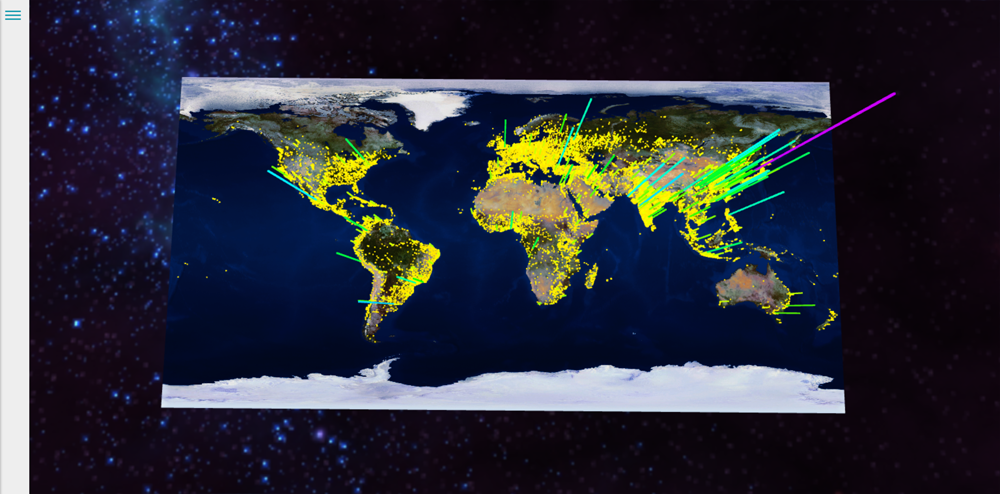
\includegraphics[width=\textwidth]{images/implementation/system/cuboid}}
	\caption{Population dataset on a cuboid surface.}
	\label{fig:cuboid_surface}
\end{figure}


	The second visualisation modified the surface and projection used in the previous implementation, which have been described in Section~\ref{sec:surface} and~\ref{sec:data_point_display}. This visualisation also used a population dataset, which can be seen in Figure~\ref{fig:sphere_surface} and hence the same processing techniques were utilised during application startup.

	%!TEX root = ../../../report.tex

\begin{figure}[H]
	\centering
	\figureborder{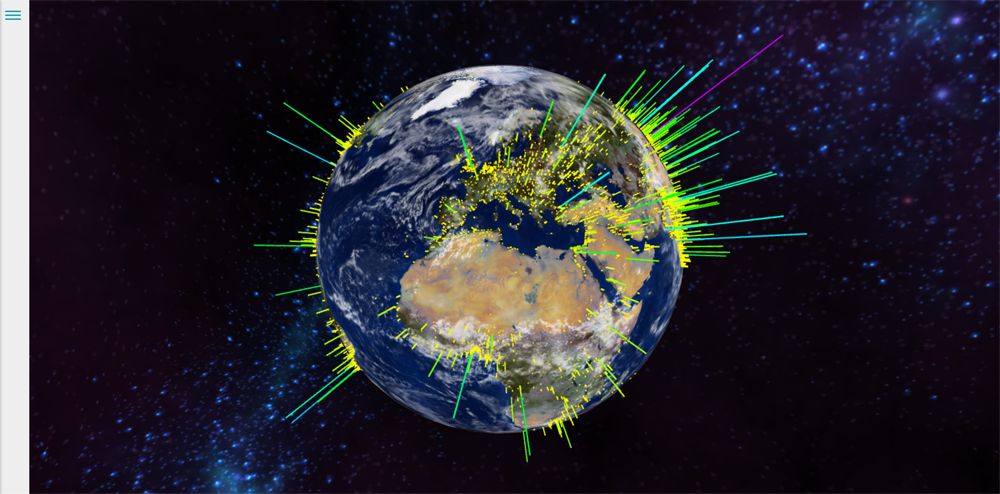
\includegraphics[width=\textwidth]{images/implementation/system/sphere}}
	\caption{Population dataset on a sphere surface.}
	\label{fig:sphere_surface}
\end{figure}


	The final implementation for this system attempts to facilitate the analysis of ongoing student progress for a tutorial as shown in Figure~\ref{fig:grid_surface}. The data in this visualisation represents the weekly progress for each student group within a case scenario. Data points indicate how much a group has progressed (e.g. Issues and Evidence) in their case activities for a particular week, where taller data points correspond to a greater value of completion.

	%!TEX root = ../../../report.tex

\begin{figure}[H]
	\centering
	\figureborder{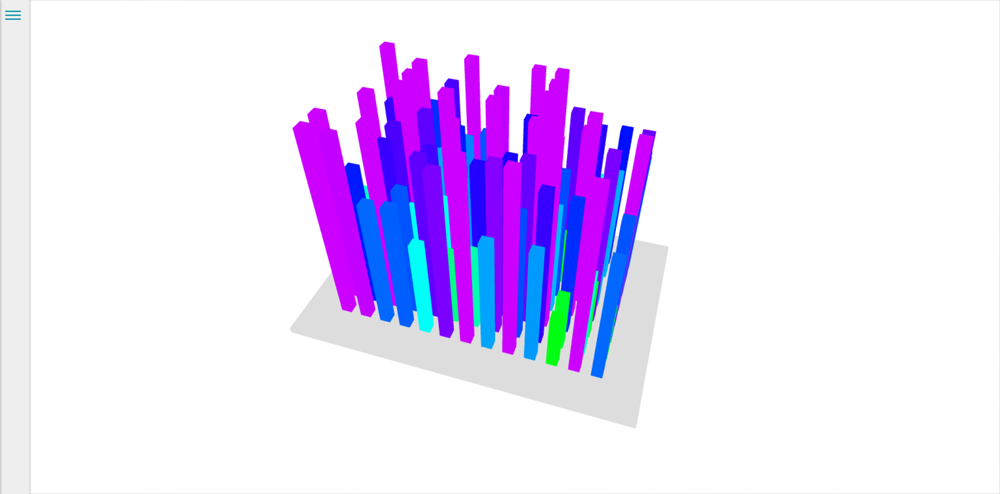
\includegraphics[width=\textwidth]{images/implementation/system/grid}}
	\caption{Student dataset on a grid surface.}
	\label{fig:grid_surface}
\end{figure}


	Furthermore, the student grid visualisation required alternate processing techniques for implementation. First of all, when the dataset was processed the $x$, $y$ and $z$ values were instead mapped to $group$, $week$ and $progress$. Since this dataset cannot map keys to the position of a point, as the data may include strings, the position had to be calculated using the $x$, $y$ and $z$ values. This is unlike the population dataset, which was able to map longitude and latitude to a position. Finally, there are two significant differences between this visualisation and the previous two that have been outlined. The first is that there is no skybox displayed in the scene and the second is that the surface does not utilise textures or shaders.
	
}

\section{Architecture} {
\label{sec:architecture}

	The system architecture for this system has been shown through a conceptual class diagram as seen in Figure~\ref{fig:conceptual_class_diagram}. For a more detailed architecture class diagram, refer to Appendix~\ref{app:architecture}.

	%!TEX root = ../../report.tex

\begin{figure}[H]
	\centering
    \includegraphics[width=\textwidth]{images/design/conceptual_class_diagram}
    \caption[Conceptual class diagram]{The system architecture shown as a conceptual class diagram.}
    \label{fig:conceptual_class_diagram}
\end{figure}


	The system is highly inheritance-based by incorporating the \texttt{THREE.Mesh} for each item in the 3D environment. An overview of the core modules has been described below:

	\begin{sloppypar}
		\begin{description}[leftmargin=0pt]
			\item [Application:] This module sets up the \texttt{THREE.Scene}, \texttt{THREE.Camera} and \texttt{THREE.WebGLRenderer} so the visualisation can be rendered in the main render loop. The Application module is also responsible for processing the dataset, loading the Visualisation and creating the Navigation, Information, Filters and Configurations modules. 
			\item[Visualisation:] A mesh that adds the Points, Surface and Skybox components as children. The Visualisation also applies the projection to each Point in the Points mesh.
			\item[Points:] The Points mesh is associated with the Points Backbone collection, which was processed in the Application module. This module simply adds a Point mesh for every model in the collection.
			\item[Point:] This mesh consists of a Point model, \texttt{THREE.BoxGeometry} and \texttt{THREE.ShaderMaterial}. The magnitude of the mesh is also converted so that it is capped to a maximum height.
			\item[Surface:] A base class that represents a mesh for the Cuboid and Sphere surfaces.
			\item[Skybox:] This mesh asynchronously loads six image resources as textures, which are then applied to each side of the cube geometry to form the appearance of the skybox.
			\item[Projection:] A class that modifies the position and rotation of an object to simulate a mathematical projection. This is achieved through a custom function, which typically applies a standard or spherical projection.
			\item[Navigation:] Listens to mouse events on the specified element, in this case the HTML5 canvas, and adjusts the position and rotation of the camera to reflect user input. The possible navigation techniques are pan, zoom and rotate.
			\item[Information:] This module listens for events in the Raycaster. It updates the view with the correct model data and recalculates the position of the display when an intersection between the mouse pointer and a data point occurs.
			\item[Filters:] Creates Slider and Checkbox view controllers based on the values in the Backbone collection. It also listens to \texttt{change} events on the sliders and their number inputs as well as the checkboxes. The event handlers for these widgets filters the data, firing a \texttt{filter} event with the filtered collection. The filter event is then caught by the Filter module, which handles the processing of the collection and in turn the visibility of the Points.
			\item[Configurations:] Initialises the real-time configuration widgets that adjust the appearance of the 3D environment. This module listens to \texttt{change} events on each input in order to update the shader uniforms for a mesh, which requires custom event handlers and conversions between units.
		\end{description}
	\end{sloppypar}

}

\section{Datasets} {
\label{sec:datasets}

	\subsection{Population dataset} {
	\label{sec:population_dataset}

		The GeoNames database was used as the basis for the population dataset. This data was preprocessed with a Python script and converted into a JSON structure, so it could be used with the visualisations. One issue with the dataset is that it does not contain the name of the country. This data could be considered important to the user, as the country associated with a data point can be identified when using the information displays. This data was added by loading a separate JSON dataset that contained a list of country names and their code, and mapping each country code to its corresponding name. The GeoNames dataset contained country codes, so the country name could be accessed with this map and added to the final output for each city. Alongside this processing, unwanted information such as elevation and administration codes were filtered out and specific strings were converted to numbers before the output was exported to a JSON file.

	}

	\subsection{Student progress dataset} {
	\label{sec:student_progress_dataset}

		The data used to monitor student progress can be retrieved from the server used in the group project. During application startup, an AJAX request is performed to fetch the data from the live system. This data is then processed and stored in a Backbone collection which is to be used with the \texttt{Grid} visualisation to create each data point.

	}

	\subsection{Structure} {
	\label{sec:dataset_structure}

		The structure used in both the population and student progress datasets has been shown in Figure~\ref{fig:datasets} below.

		%!TEX root = ../../report.tex

\begin{figure}[H]
	\newcommand{\figurewidth}{0.5\textwidth}
	\begin{subfigure}[b]{\figurewidth}
		\centering
		%!TEX root = ../../report.tex

\begin{lstlisting}
	{
		"city": String,
		"country": String,
		"country_code": String,
		"latitude": Number,
		"longitude": Number,
		"modification_date": String,
		"population": Number
	}
\end{lstlisting}
		
		\caption{Structure of the population dataset.}
		\label{fig:population_dataset_structure}
	\end{subfigure}
	\begin{subfigure}[b]{\figurewidth}
		\centering
		%!TEX root = ../../report.tex

\begin{lstlisting}
	{
		"week": Number,
		"tutorial": String,
		"case": String,
		"group": String,
		"activity": String,
		"progress": Number,
		"complete": Boolean
	}
\end{lstlisting}

		\caption{Structure of the student dataset.}
		\label{fig:student_dataset_structure}
	\end{subfigure}
	\caption[Dataset structures]{The structures used for both datasets.}
	\label{fig:datasets}
\end{figure}


	}

}

\section{Navigation} {
\label{sec:navigation}

	The navigation techniques that the user can interact with are pan, rotate and zoom. This functionality was implemented in a single module and utilised mouse events to detect when the user was scrolling or pressing the left or right mouse button. It is important to note that Three.js uses a right-handed coordinate system, as shown in Figure~\ref{fig:threejs_coordinate_system}.

	%!TEX root = ../../report.tex

\begin{figure}[H]
	\centering
	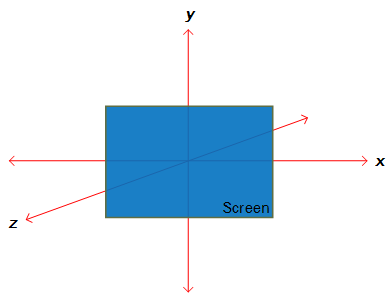
\includegraphics{images/implementation/threejs_coordinate_system}
	\caption[Three.js coordinate system]{Three.js coordinate system\protect\footnotemark.}
	\label{fig:threejs_coordinate_system}
\end{figure}

\footnotetext{\bibentry{microsoft2015threejs}}


	\subsection{Pan} {
	\label{sec:pan}

		This interaction is initiated when a \texttt{mousedown} event is fired on the canvas, followed by a \texttt{mousemove} event bound to the \texttt{window}. This simulates drag when pressing the left mouse button.

		As the user moves their pointer, the camera is translated in the x and y direction. This calculation relies on converting screen coordinates to world coordinates and normalising the value so it is a ratio of the viewport height, instead of both the width and height.

		Once the translation to the camera has been applied, the \texttt{origin} vector needs to be updated, which is used during rotation. An updated origin ensures there is no sudden movement when rotating, after panning the screen.

		Finally, when the user releases the left mouse button, a \texttt{mouseup} event is triggered which removes the event binding for \texttt{mousemove} on the \texttt{window}. 

	}

	\subsection{Rotate} {
	\label{sec:rotate}

		Rotation uses the same event chain as panning, except instead of listening to the left mouse click, it listens to the right.

		To rotate the camera, the cartesian coordinates need to be calculated from spherical coordinates, using the following formula in a right-handed mathematics system:

		%!TEX root = ../../report.tex

\begin{gather*}
	x = r\sin\phi\sin\theta \\
	y = r\cos\phi \\
	z = r\sin\phi\cos\theta
	\intertext{Where:}
	\begin{tabularx}{\textwidth}{@{}>{$}r<{$}@{\ :\ }X@{}}
		r & is the radial distance of the camera from the origin. \\
		\phi & is the polar angle, calculated by adding the delta phi angle with the angle from the y-axis. \\
		\theta & is the azimuthal angle, calculated by adding the delta theta angle with the angle from the z-axis around the y-axis. \\
	\end{tabularx}
\end{gather*}
	
	}

	\subsection{Zoom} {
	\label{sec:zoom}

		This navigation technique begins when the user scrolls with their mouse, triggering a \texttt{wheel} event in the browser. A ratio of the delta value is taken and the camera is then translated by this amount.
	
	}

}

\section{Surface} {
\label{sec:surface}

	\begin{sloppypar}
		A surface consists of a \texttt{THREE.Mesh} and uses either a \texttt{THREE.BoxGeometry} or \texttt{THREE.SphereGeometry} for its geometry. The material used in both the cuboid and sphere surface is a \texttt{THREE.ShaderMaterial}, which facilitates the configuration of midtone effects and other uniforms. The entry point for the shader using the GLSL language is demonstrated below.
	\end{sloppypar}

	%!TEX root = ../../report.tex

\begin{lstlisting}[language=GLSL]
	void main() {
		if (vPosition.y < uSurfacePosition) {
			gl_FragColor = vec4(uColor, 1.0);
		} else {
		    vec3 originalColor = texture2D(uTexture, vUv).rgb;
		    vec3 colorShift = vec3(uRedShift, uGreenShift, uBlueShift);
		    vec3 color = colorBalance(originalColor, colorShift);

			gl_FragColor = vec4(color, 1.0);
		}
	}
\end{lstlisting}


	The above snippet of code applies a colour balance effect to every point in the fragment shader that represents the surface texture. In a cuboid surface for instance, any point that is beneath the top face is set to a solid colour. This removes the appearance of a stretched texture on all other sides of the cuboid. In contrast to this, the grid surface uses a simple \texttt{THREE.MeshBasicMaterial} as it does not contain a texture or other uniforms.

}

\section{Data point display} {
\label{sec:data_point_display}

	The data point displays were implemented by creating a \texttt{THREE.Mesh} that acts as a \texttt{Points} container for all \texttt{Point} meshes. The \texttt{Points} class is repsonsible for creating all of the data point displays, using the \texttt{Point} Backbone collection created and populated with information from the dataset during application startup. Each model in this collection specifies the initial position and magnitude of the \texttt{Point} mesh, which consists of a \texttt{THREE.BoxGeometry} and \texttt{THREE.ShaderMaterial}. Additionally, the \texttt{Visualisation} class ensures that each \texttt{Point} in the \texttt{Points} mesh appears as if it were on top of the surface, by applying either a standard for cuboids or a spherical projection for spheres.

	The standard projection simply sets the y-position of the object by some offset, in this case the height of the cuboid surface, and then converts the range of the x and z-positions so that is fits on the cuboid dimensions. Whereas the spherical projection first converts x-position of the object to $\theta$ and the z-position to $\phi$ in radians. These values are used, along with the radius of the sphere, to apply a spherical to cartesian conversion which denotes the position of the \texttt{Point}. Then, the point is rotated to face the position of the sphere and again in the x-direction so it is not tangential to the surface.

	Further, the shader used as the shader material in the \texttt{Point} class uses various uniforms to provide a multitude of configurable effects to the user. One important aspect of the data displays is their ability to change their appearance from a Hue, Saturation and Value (HSV) colour range to a gradient colour scheme, which can be seen in Figure~\ref{fig:data_point_displays} below. This has been completed with a simple fragment shader that changes which scheme to use for the display of the data points. The following code demonstrates the main entry point of this shader:

	%!TEX root = ../../report.tex

\begin{lstlisting}[language=GLSL,basicstyle=\scriptsize\ttfamily]
	vec3 basicColor(vec2 uBound, vec2 uColorRange, float uMagnitude, float uSaturation, float uLightness) {
		float hue = clamp(convertRange(uBound, uColorRange, uMagnitude), 0.0, 1.0);
		return hsv2rgb(vec3(hue, uSaturation, uValue));
	}

	vec3 gradientColor(vec2 uBound, vec3 vPosition, vec3 uLowColor, vec3 uMediumColor, vec3 uHighColor) {
		// Calculate the bound and colour stop.
		float bound = abs(uBound.y - uBound.x);
		float colorStop = bound * 0.3;
		// Get the current y position of the vertex.
		float y = vPosition.y;
		// Return the gradient colour.
	    return mix(mix(uLowColor, uMediumColor, smoothstep(uBound.x, colorStop, y)), uHighColor, smoothstep(colorStop, uBound.y, y));
	}

	void main() {
		vec3 color;
		if (uMode == 0) {
			color = basicColor(uBound, uColorRange, uMagnitude, uSaturation, uValue);
		} else {
			color = gradientColor(uBound, vPosition, uLowColor, uMediumColor, uHighColor);
		}
		gl_FragColor = vec4(color, uAlpha);
	}
\end{lstlisting}


	%!TEX root = ../../report.tex

\begin{figure}[H]
	\captionsetup[subfigure]{aboveskip=-0.8em,belowskip=0.5em}
	\newcommand{\figurewidth}{0.5\textwidth}
	\begin{subfigure}[b]{\figurewidth}
        \figureborder{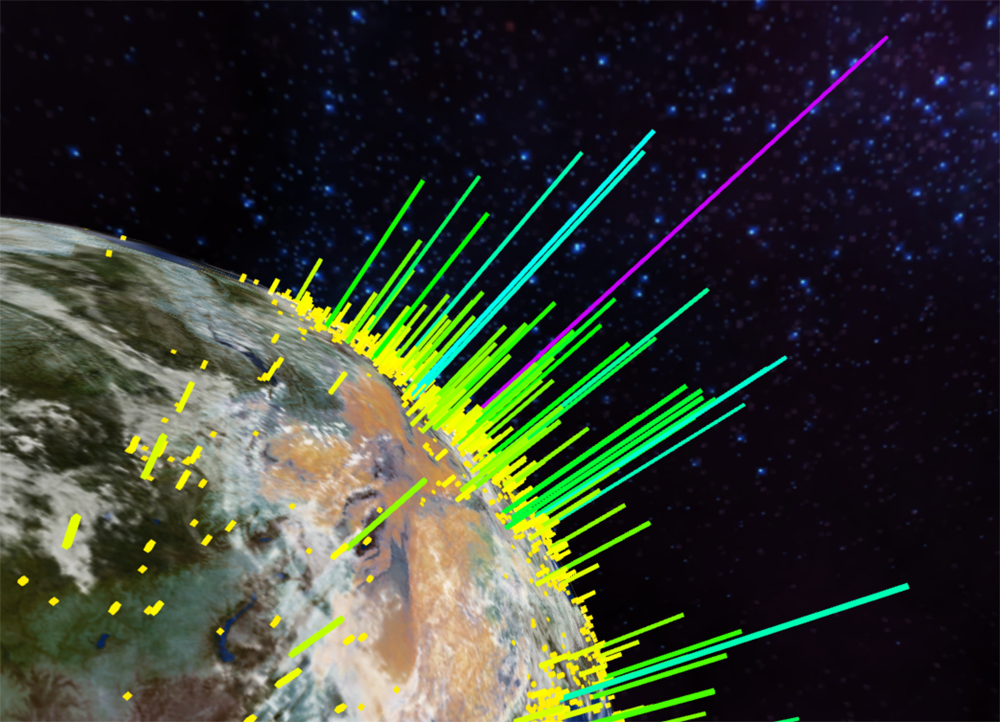
\includegraphics[width=\textwidth]{images/implementation/data_display/basic}}
		\caption{Basic shader data point display.}
		\label{fig:basic_shader}
	\end{subfigure}
	\begin{subfigure}[b]{\figurewidth}
		\figureborder{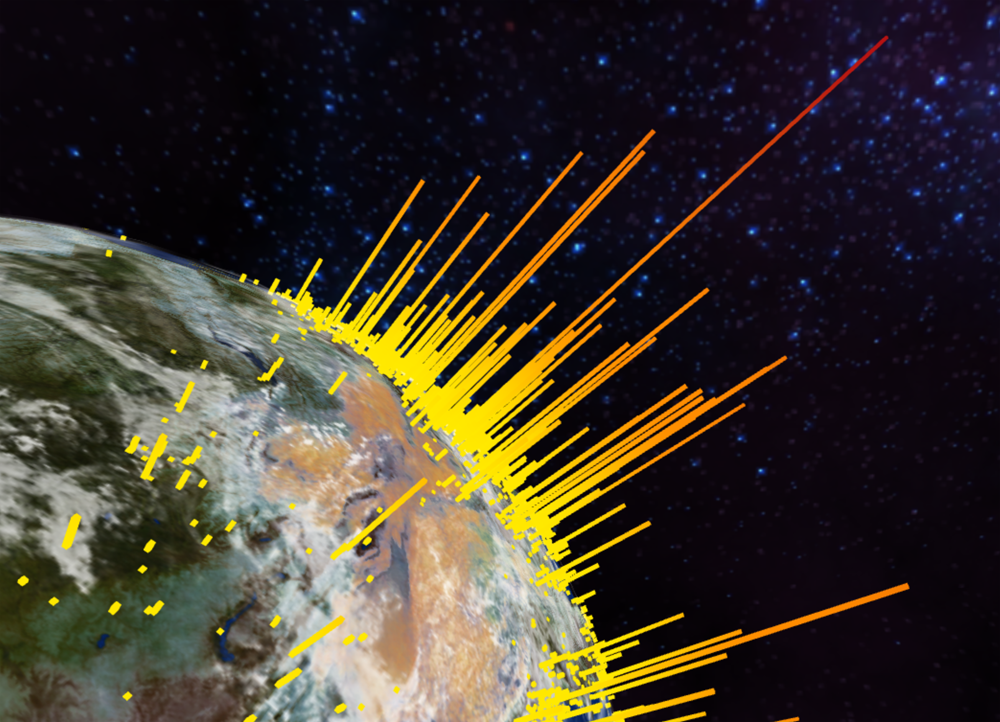
\includegraphics[width=\textwidth]{images/implementation/data_display/gradient}}
		\caption{Gradient shader data point display.}
		\label{fig:gradient_shader}
	\end{subfigure}
	\caption[Data point display types]{Types of data point displays.}
	\label{fig:data_point_displays}
\end{figure}


}

\section{Information display} {
\label{sec:information_display}

	The information display utilises a \texttt{THREE.Raycaster} and a Handlebars template for displaying model information. The raycaster is updated on each render loop and is fed a series of \texttt{Point} meshes to check if the normalised mouse coordinates intersect with any data points. These intersections are listened to in the \texttt{Information} view controller, which is responsible for updating the content and visibility of the information display element. A single element has been used to display this information as the creation of DOM elements is incredibly inefficient, especially because this would entail creating an element for each intersection at run-time. When an intersection exists, the element is displayed and its HTML is updated with its model data through Handlebars. Further, the \texttt{left} and \texttt{top} position of the element is updated to match the mouse coordinates. The position of the element is improved by calculating the quadrant in which the coordinate lies and adjusting the position such that the display is always towards the centre of the screen. This prevents the information from being clipped off when the user hovers at the edge of the screen. An example of this and the design of the information display hover effect can be seen in Figure~\ref{fig:information_display}.

	%!TEX root = ../../report.tex

\begin{figure}[H]
	\centering
	\newcommand{\figurewidth}{0.4\textwidth}
	\centering
	\begin{subfigure}[b]{\figurewidth}
        \figureborder{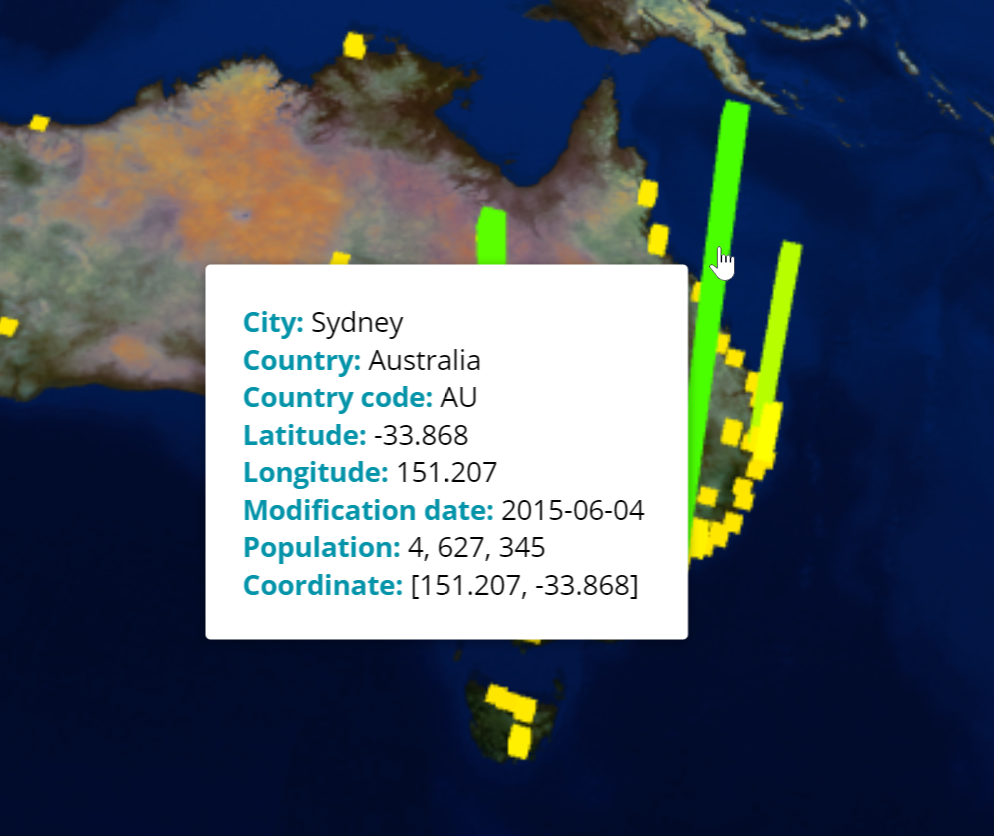
\includegraphics[width=\textwidth]{images/implementation/information_display/population}}
		\caption{Information display for population data.}
		\label{fig:information_display_population}
	\end{subfigure}
	\begin{subfigure}[b]{\figurewidth}
		\figureborder{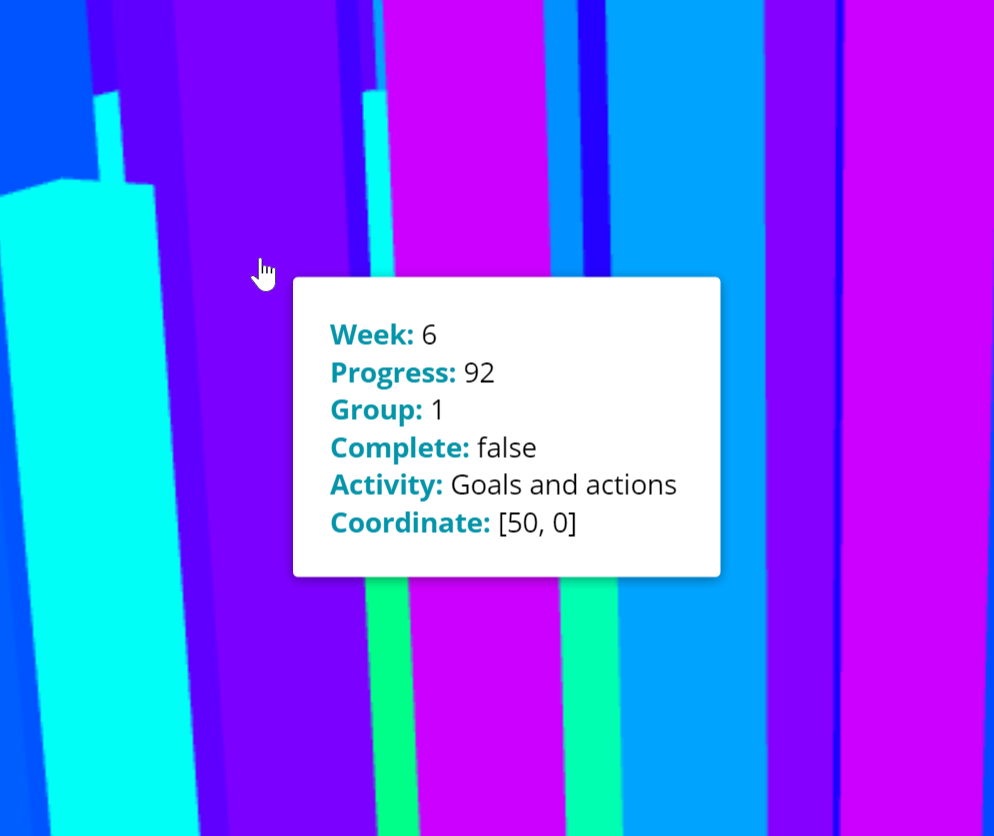
\includegraphics[width=\textwidth]{images/implementation/information_display/student}}
		\caption{Information display for student data.}
		\label{fig:information_display_student}
	\end{subfigure}
	\caption[Information display]{Information display hover effect.}
	\label{fig:information_display}
\end{figure}


}

\section{Skybox} {
\label{sec:skybox}

	The skybox was generated using \href{http://alexcpeterson.com/spacescape/}{Spacescape}, a program designed for creating space skyboxes with stars and nebulas. Once the skybox was created, the images were exported as six individual images. The formation of these images can be seen in Figure~\ref{fig:skybox}.

	%!TEX root = ../../report.tex

\begin{figure}[H]
	\centering
	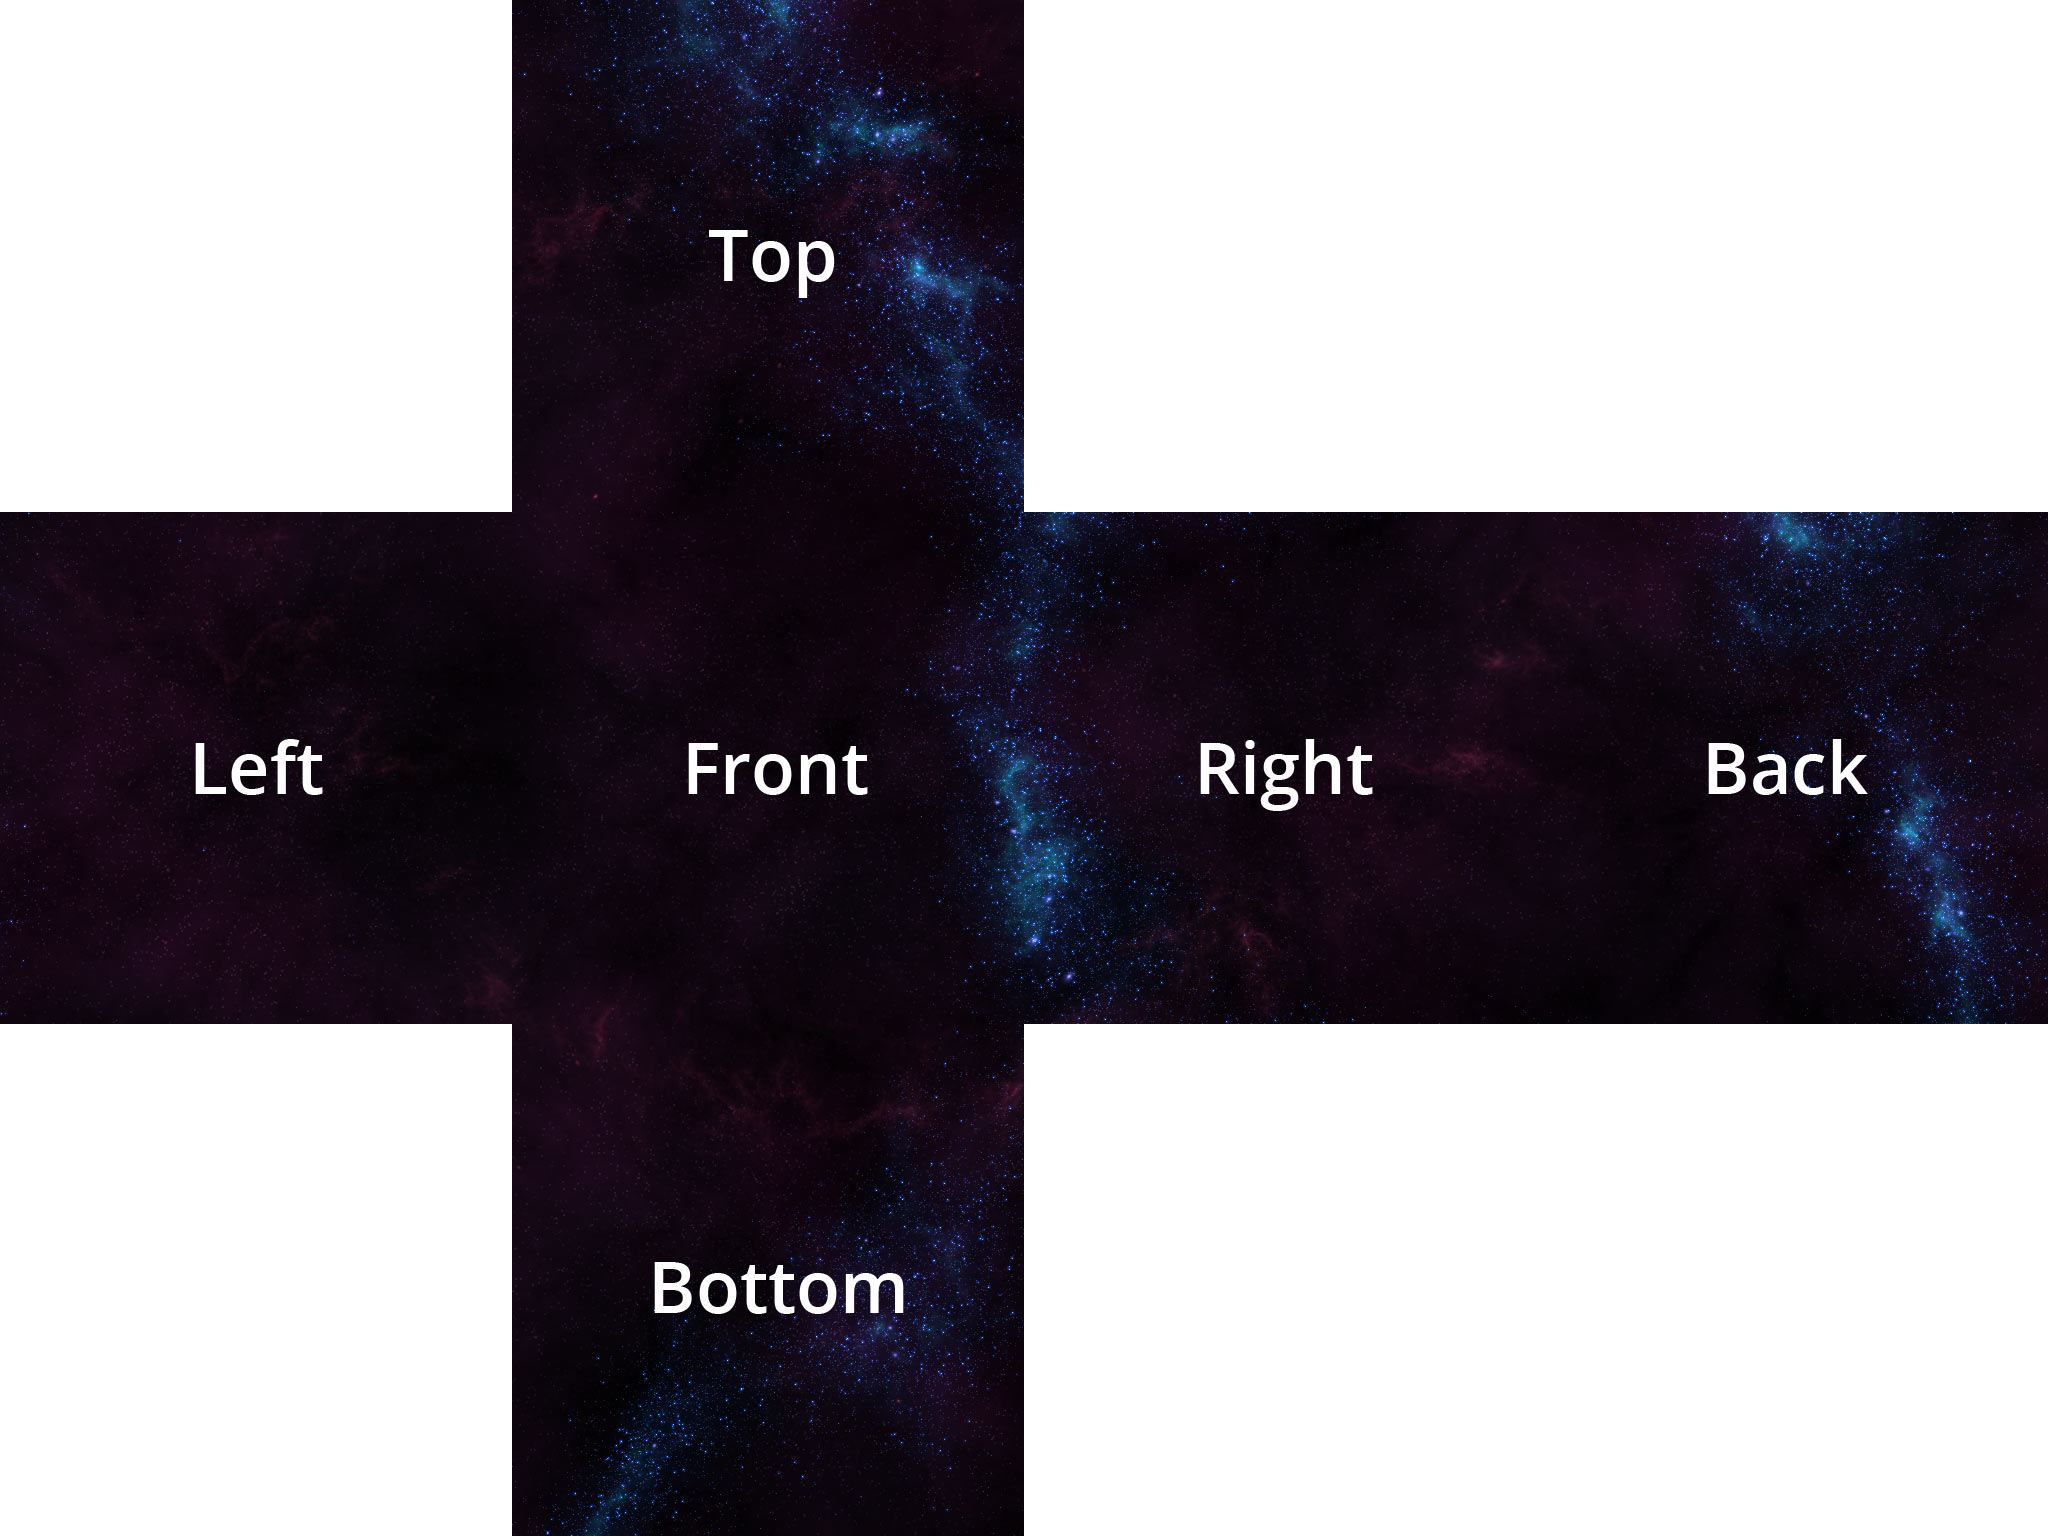
\includegraphics[width=0.6\textwidth]{images/implementation/skybox}
	\caption[Skybox]{The six images used for the skybox and their positions.}
	\label{fig:skybox}
\end{figure}


	\begin{sloppypar}
		The implementation of the skybox was a simple process. This process involved loading each side of the cuboid as a \texttt{THREE.Texture} and assigning it as a \texttt{map} in a \texttt{THREE.MeshBasicMaterial} object. Each basic material was stored in an array, so that the skybox mesh could be created using a \texttt{THREE.BoxGeometry} and \texttt{THREE.MeshFaceMaterial}. It is important that the skybox is static during navigation, particularly so that the underlying cuboid structure of the skybox is not noticeable and appears more realistic to the user. This was accomplished by listening to the \texttt{pan}, \texttt{zoom} and \texttt{rotate} events in the mouse controls, and updating the position of the skybox to reflect that of the camera.
	\end{sloppypar}

}

\section{Drawer menu} {
\label{sec:drawer}

	The drawer menu is located on the left side of the system and is initially closed to maximise the visualisation viewing area. It has been built with pure CSS, using a checkbox that alters and transitions the position of the menu when the checkbox is checked. This interface has been shown in Figure~\ref{fig:drawer} below.

	%!TEX root = ../../report.tex

\begin{figure}[H]
	\newcommand{\figurewidth}{0.5\textwidth}
	\begin{subfigure}[b]{\figurewidth}
        \figureborder{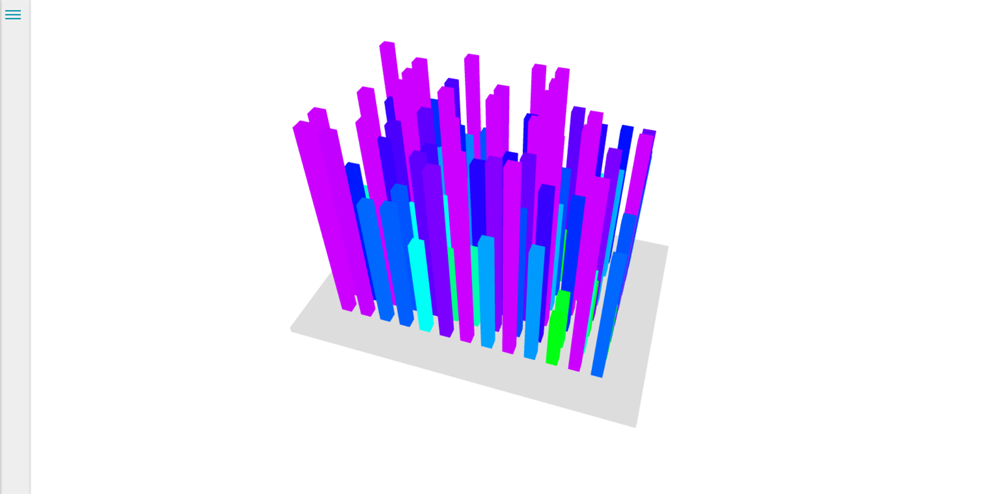
\includegraphics[width=\textwidth]{images/implementation/drawer/closed}}
		\caption{Closed drawer.}
		\label{fig:closed_drawer}
	\end{subfigure}
	\begin{subfigure}[b]{\figurewidth}
		\figureborder{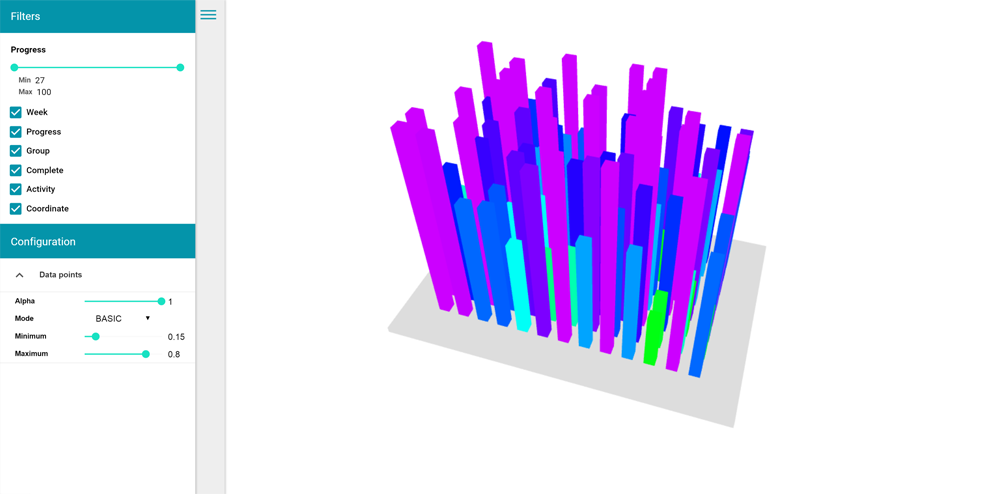
\includegraphics[width=\textwidth]{images/implementation/drawer/open}}
		\caption{Open drawer.}
		\label{fig:open_drawer}
	\end{subfigure}
	\caption{Drawer interface.}
	\label{fig:drawer}
\end{figure}


}

\section{Filtering} {
\label{sec:filtering_implementation}

	Filtering was implemented using an event-driven approach and a view controller for configuring the filters. This view controller comprises the slider and checkbox views, which were designed using Handlebars templates and populated with a Backbone model. The final design of this interface has been demonstrated in Figure~\ref{fig:filtering_interface}.

	%!TEX root = ../../../report.tex

\begin{wrapfigure}[13]{r}{0.4\textwidth}
	\captionsetup{aboveskip=0em}
	\vspace{-2.5em}
	\begin{center}
		\figureborder{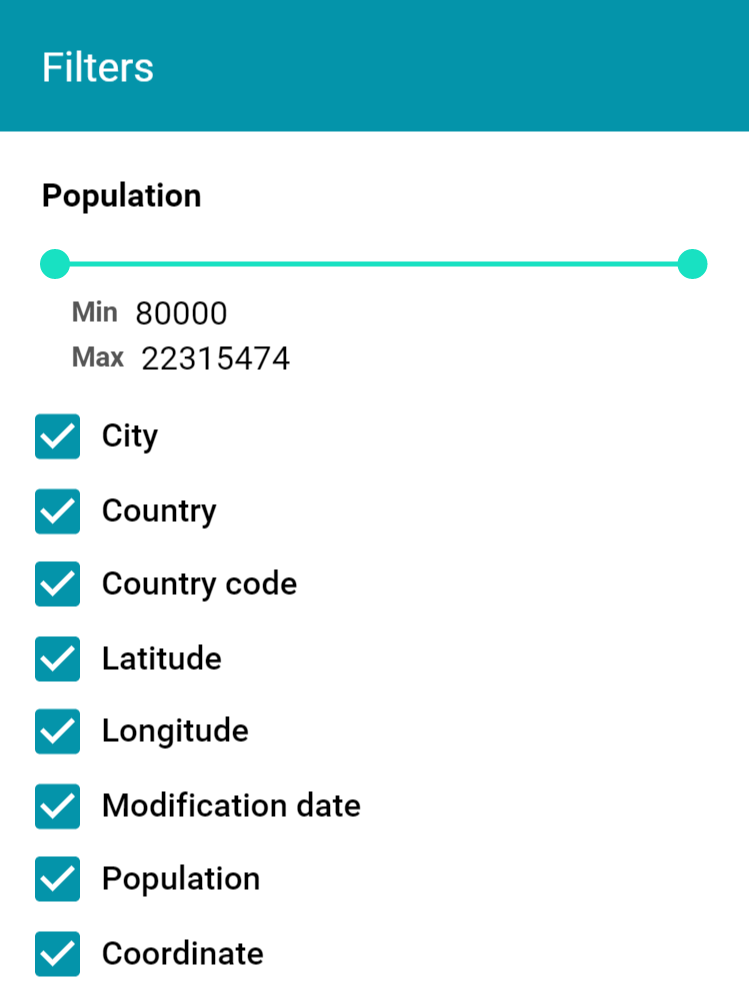
\includegraphics[width=0.4\textwidth]{images/implementation/filtering/interface}}
	\end{center}
	\caption[Filtering]{Filtering interface.}
	\label{fig:filtering_interface}
\end{wrapfigure}


	As a user adjusts the values in the slider, an \texttt{update} event is triggered. When this occurs, the event handler adjusts the minimum and maximum input to reflect the new slider widget values. Then, the Backbone collection that represents the data displays are filtered by calling the \texttt{filterBy} function with a filter function. This method is reposnsible for iterating through each model in the collection and determining if it should be filtered. A simple example of a filter function is:

	%!TEX root = ../../report.tex

\begin{lstlisting}
	function (model) {
		let value = model.get(property);
		return !(value > min && value <= max);
	}
\end{lstlisting}


	The above function utilises closure to check if the property associated with the slider is within the specified minimum and maximum bounds. If this function returns \texttt{true}, the model is added to a filtered collection. Once the collection has been iterated through, the \texttt{filterBy} function triggers a \texttt{filter} event with the filtered collection. The visibility of the data display mesh can then be modified based on the results of filtering.

	A similar process occurs when the user enters a value into the minimum or maximum inputs. A \texttt{keyup} event is bound to both inputs and a timer is in place to enforce a filtering delay. This delay ensures that filtering is processed as required, when the user has stopped typing, in order to reduce performance issues. When the user stops typing, the slider values are updated to match the input and filtering then proceeds as normal.

	As previously mentioned, the checkboxes represent what information is available to the user when hovering on a data display. The state of visibility for any given property is configured through a custom Handlebars helper method. This helper method is called when the information display template is updated, which is every time the user hovers on a data display. The helper method simply checks if a property is currently in a filtered list and displays the property when it is not a member of this list. So in order to configure the visibility of properties in the information display, a \texttt{change} event is bound to each chexkbox that updates the contents of the filtered list.

	The sequence of images displayed in Figure~\ref{fig:filtering_comparison} presents a comparison between the results of filtering for both data displays and information displays. From this, it can be seen that the user activities outlined in Section~\ref{sec:user_actions} have the potential to be fulfilled more quickly when there is less data to navigate through.

	%!TEX root = ../../../report.tex

\begin{figure}[H]
	\captionsetup[subfigure]{aboveskip=8pt,belowskip=8pt}
	\newcommand{\figurewidth}{0.5\textwidth}
	\begin{subfigure}[b]{\figurewidth}
		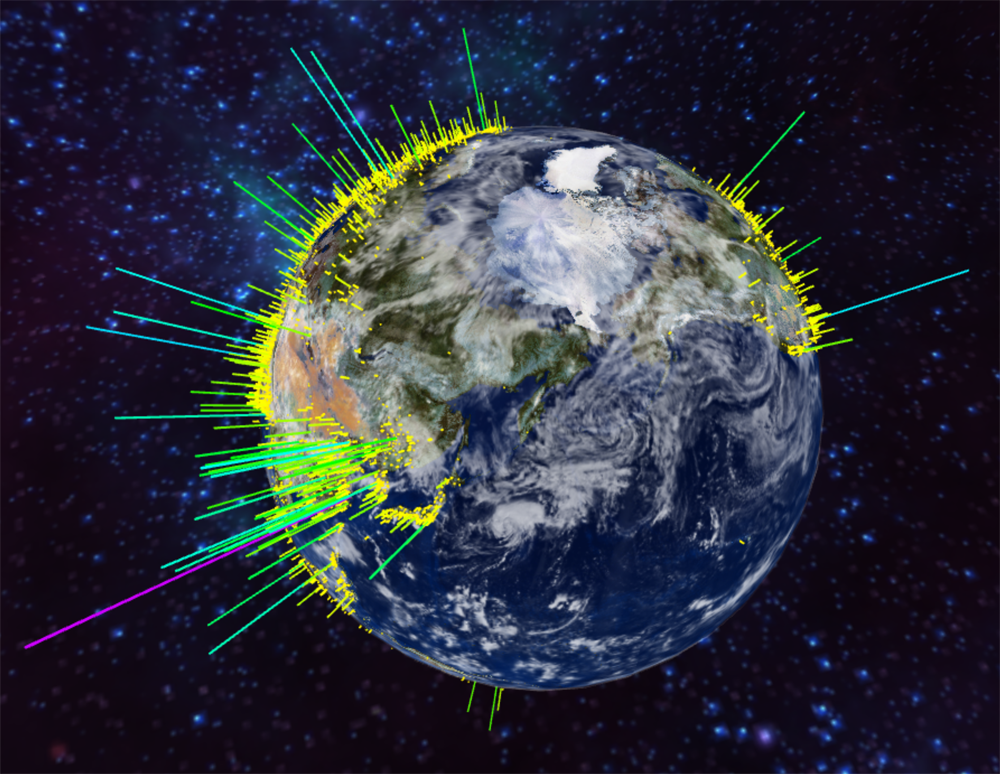
\includegraphics[width=\textwidth]{images/implementation/filtering/magnitude_before}
		\caption{Before filtering the magnitude.}
		\label{fig:before_filtering_magnitude}
	\end{subfigure}
	\begin{subfigure}[b]{\figurewidth}
		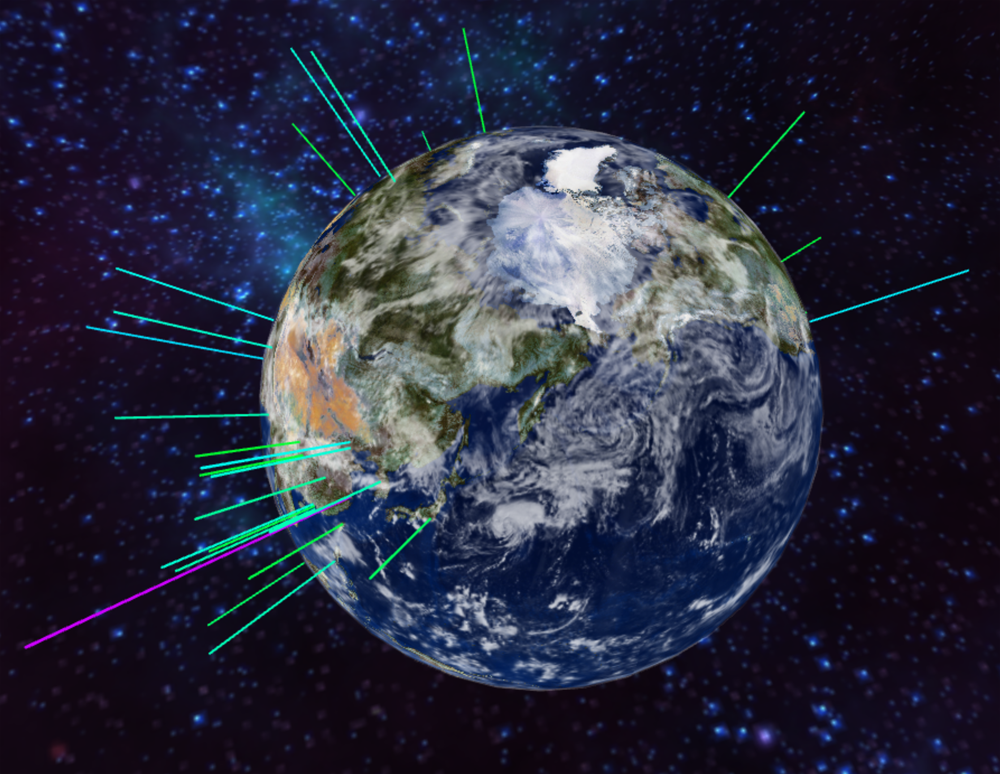
\includegraphics[width=\textwidth]{images/implementation/filtering/magnitude_after}
		\caption{After filtering the magnitude}
		\label{fig:after_filtering_magnitude}
	\end{subfigure}
	\begin{subfigure}[b]{\figurewidth}
		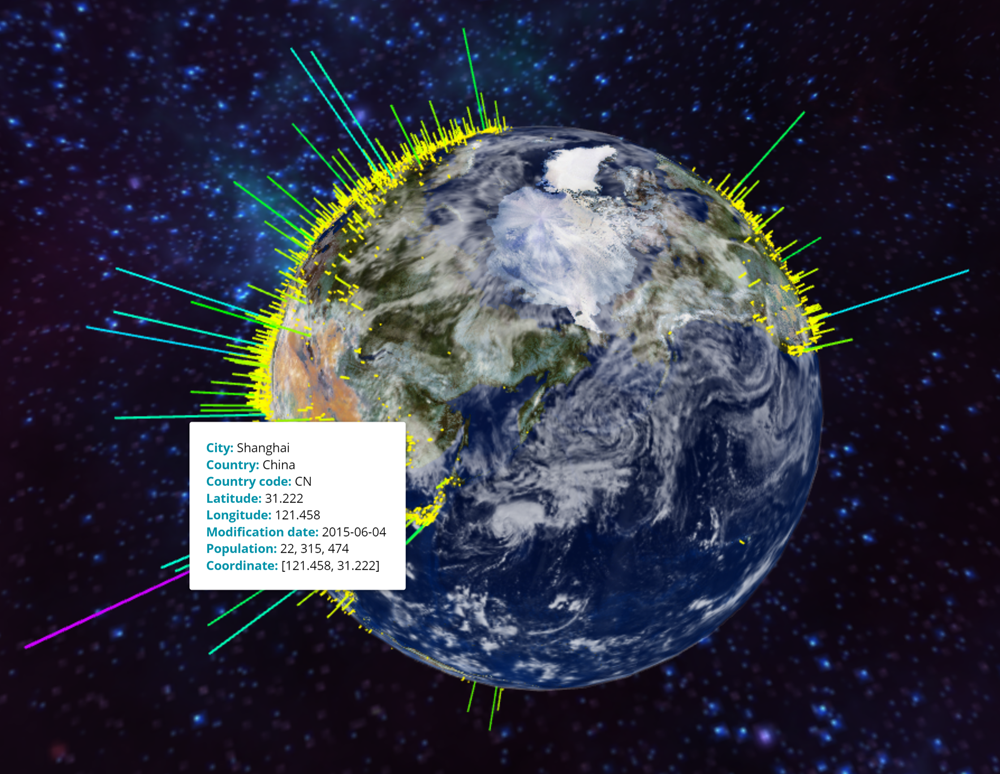
\includegraphics[width=\textwidth]{images/implementation/filtering/information_before}
		\caption{Before filtering information.}
		\label{fig:before_filtering_information}
	\end{subfigure}
	\begin{subfigure}[b]{\figurewidth}
		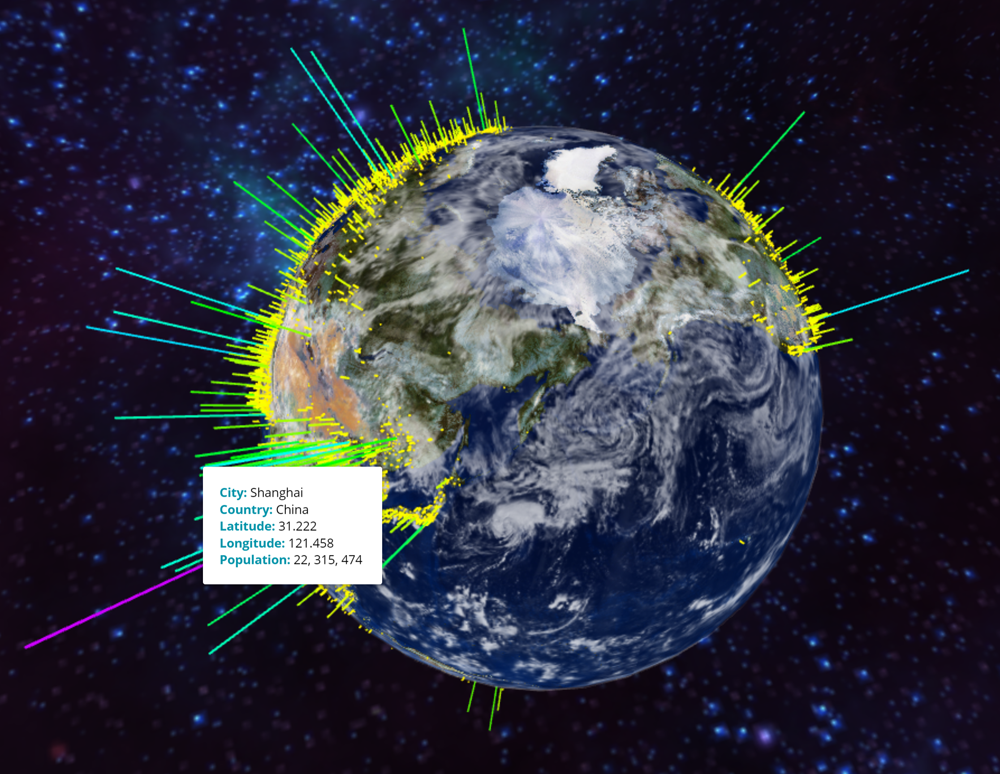
\includegraphics[width=\textwidth]{images/implementation/filtering/information_after}
		\caption{After filtering information.}
		\label{fig:after_filtering_information}
	\end{subfigure}
	\caption[Filtering comparison]{Filtering comparison.}
	\label{fig:filtering_comparison}
\end{figure}


}

\section{Configurations} {
\label{sec:configurations}

	Real-time configurations that modify the appearance of the visualisation are best achieved by using shaders. Shaders are computer programs that perform shading on a graphics processing unit (GPU), making them highly efficient and well suited to parallel processing~\footnote{\bibentry{gerdelan2014shaders}}. Three.js provides abstracted materials that use shaders in the background, but this method does not easily facilitate highly customisable configurations or filter effects. Therefore, custom shaders were designed and implemented for the system to maximise efficiency and flexibility. An example of the available effects that were implemented in the system is shown in Figure~\ref{fig:shaders}.

	%!TEX root = ../../report.tex

\begin{figure}[H]
	\captionsetup[subfigure]{aboveskip=-0.8em,belowskip=0.5em}
	\newcommand{\figurewidth}{0.5\textwidth}
	\begin{subfigure}[b]{\figurewidth}
        \figureborder{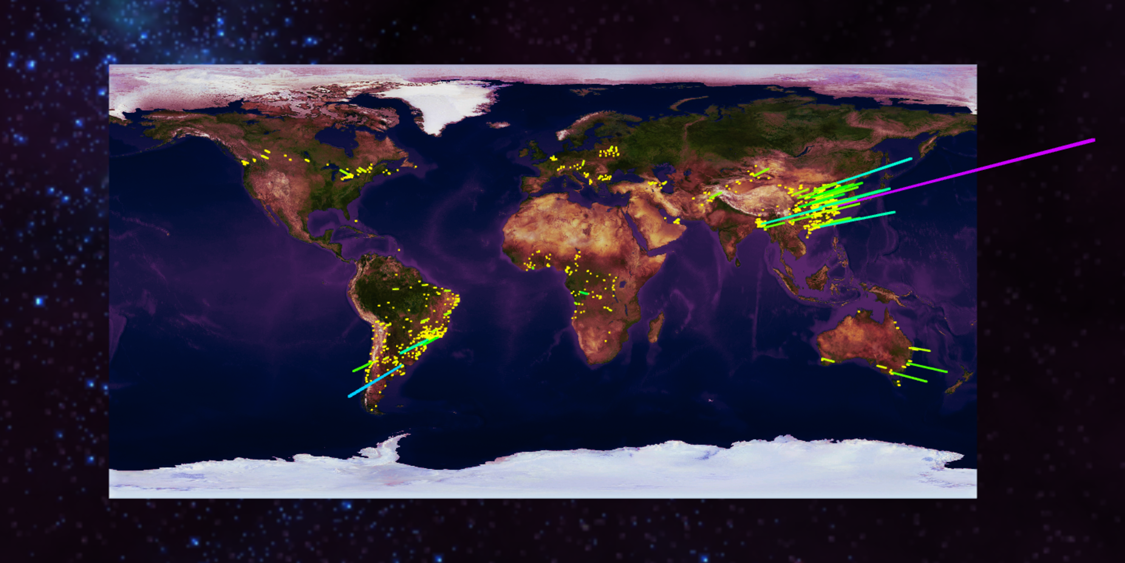
\includegraphics[width=\textwidth]{images/implementation/shaders/red}}
		\caption{Red midtone filter effect.}
		\label{fig:red_midtone}
	\end{subfigure}
	\begin{subfigure}[b]{\figurewidth}
		\figureborder{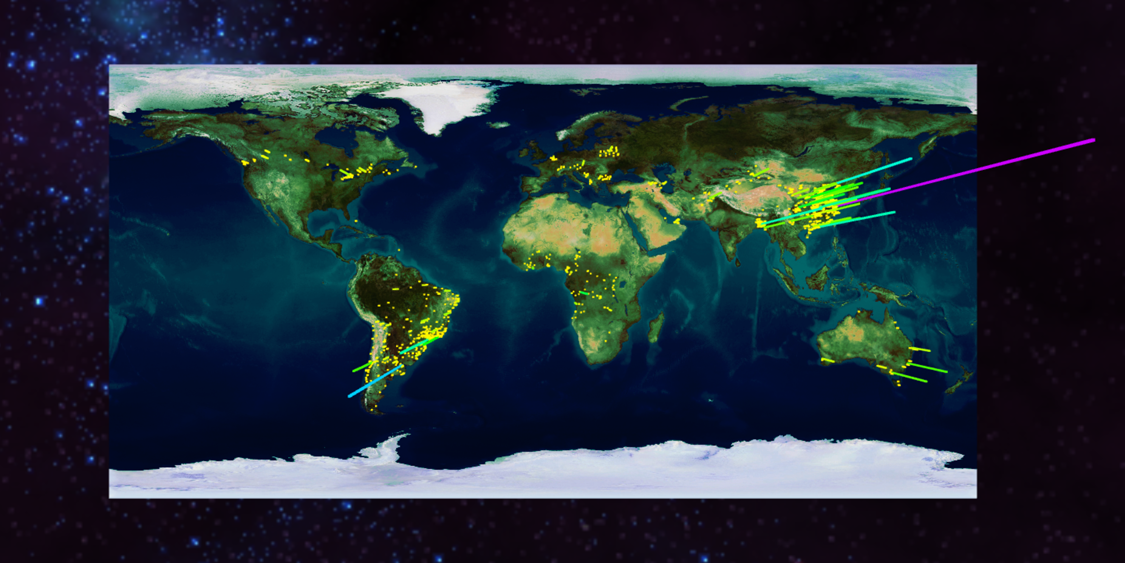
\includegraphics[width=\textwidth]{images/implementation/shaders/green}}
		\caption{Green midtone filter effect.}
		\label{fig:green_midtone}
	\end{subfigure}
	\begin{subfigure}[b]{\figurewidth}
		\figureborder{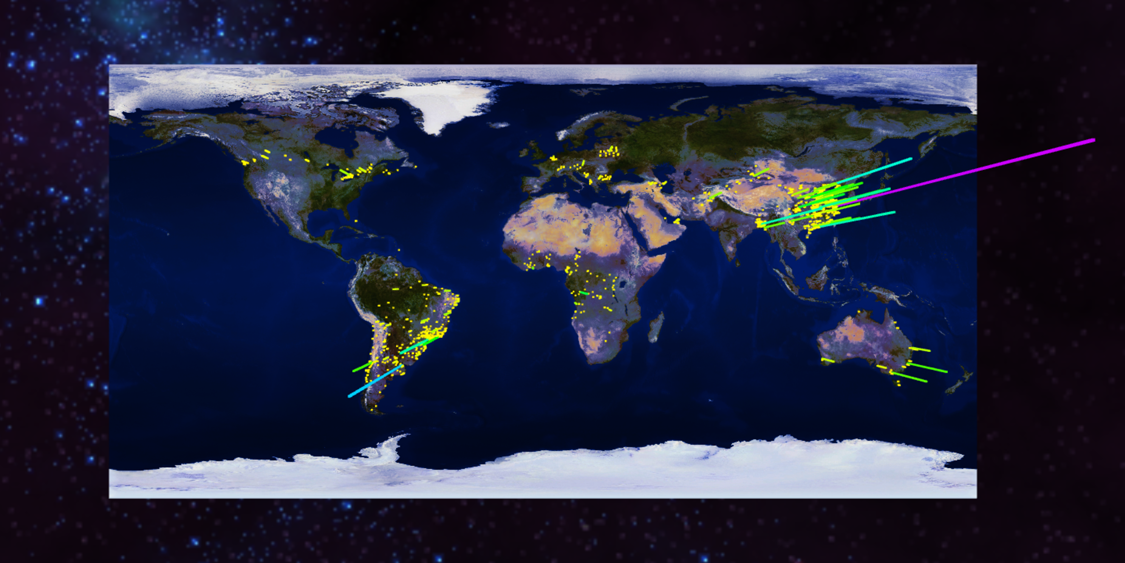
\includegraphics[width=\textwidth]{images/implementation/shaders/blue}}
		\caption{Blue midtone filter effect.}
		\label{fig:blue_midtone}
	\end{subfigure}
	\begin{subfigure}[b]{\figurewidth}
		\figureborder{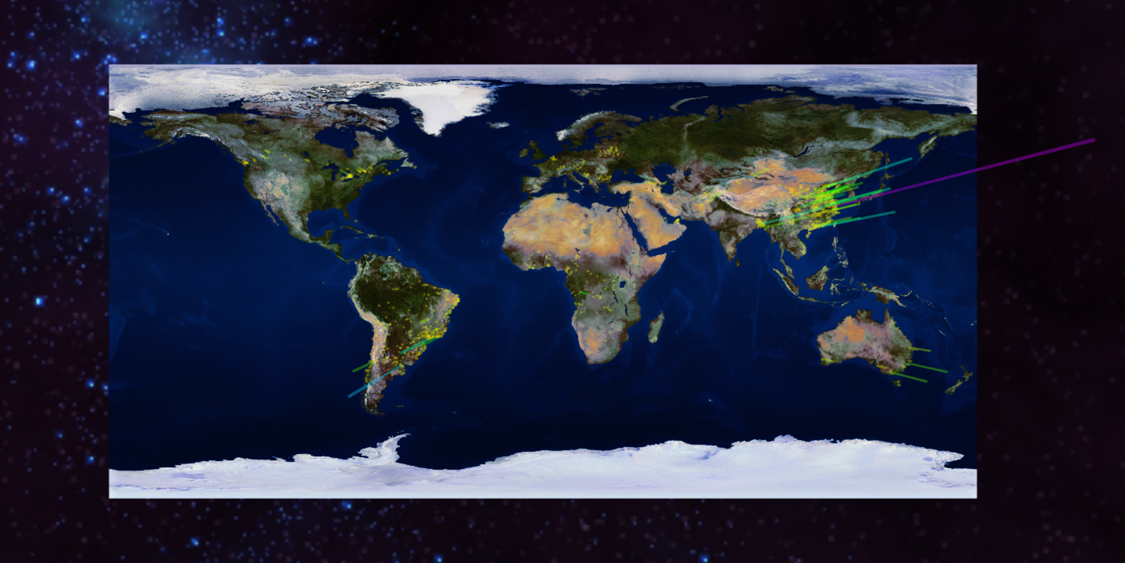
\includegraphics[width=\textwidth]{images/implementation/shaders/opacity}}
		\caption{Opacity filter effect.}
		\label{fig:opacity_filter}
	\end{subfigure}
	\begin{subfigure}[b]{\figurewidth}
		\figureborder{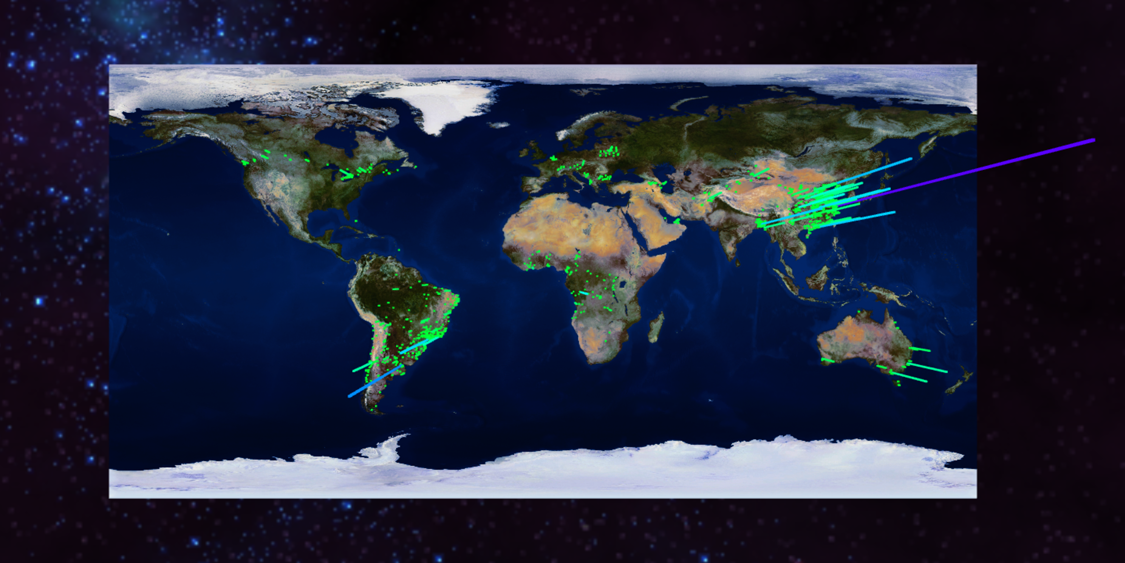
\includegraphics[width=\textwidth]{images/implementation/shaders/basic}}
		\caption{Alternate HSV colour range.}
		\label{fig:hsv_colour}
	\end{subfigure}
	\begin{subfigure}[b]{\figurewidth}
		\figureborder{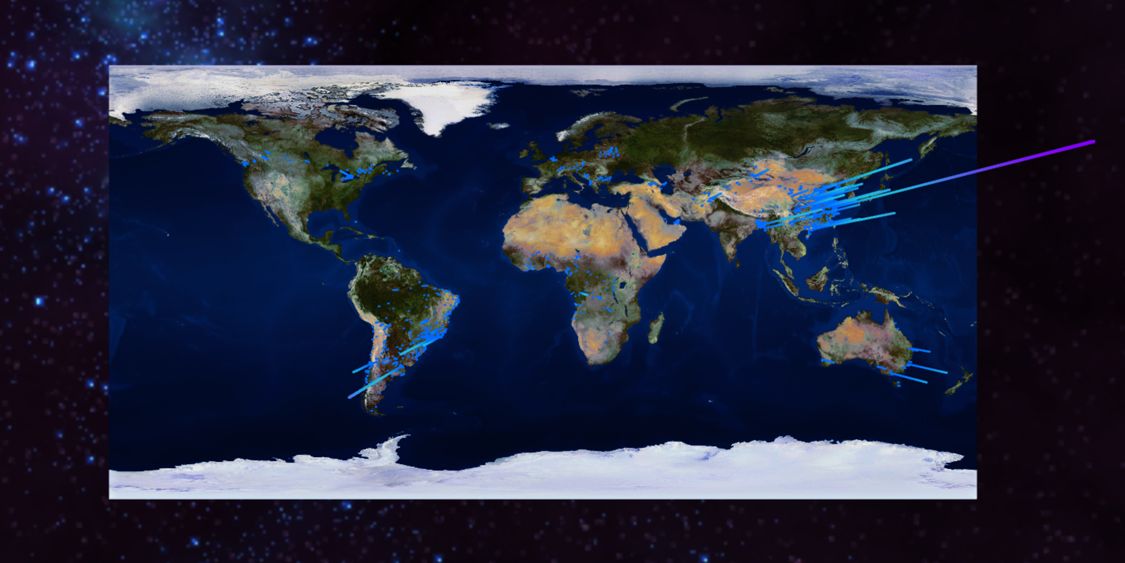
\includegraphics[width=\textwidth]{images/implementation/shaders/gradient}}
		\caption{Alternate gradient colour scheme.}
		\label{fig:gradient_colour}
	\end{subfigure}
	\caption[Shaders]{Available shader filter effects.}
	\label{fig:shaders}
\end{figure}


	These configurations can be adjusted in real-time with \href{http://workshop.chromeexperiments.com/}{dat.GUI}, a lightweight GUI for changing JavaScript variables in real-time. This tool is easy to use, setup and can modify shader uniforms automatically or by implementing \texttt{onChange} event handlers. dat.GUI can constrain input data and provides widgets for modifying values, colours and combo boxes. While this tool is great for modifying data on the fly, it has an outdated interface that does not always adapt well to particular colour schemes and designs. For this reason, the dat.GUI styles were modified to seamlessly integrate with the current system and the Material Design standards. The differences in design can be compared in Figure~\ref{fig:dat_gui} below.

	%!TEX root = ../../report.tex

\begin{figure}[H]
	\newcommand{\figurewidth}{0.4\textwidth}
	\newcommand{\figureheight}{7cm}
	\centering
	\begin{subfigure}[b]{\figurewidth}
        \figureborder{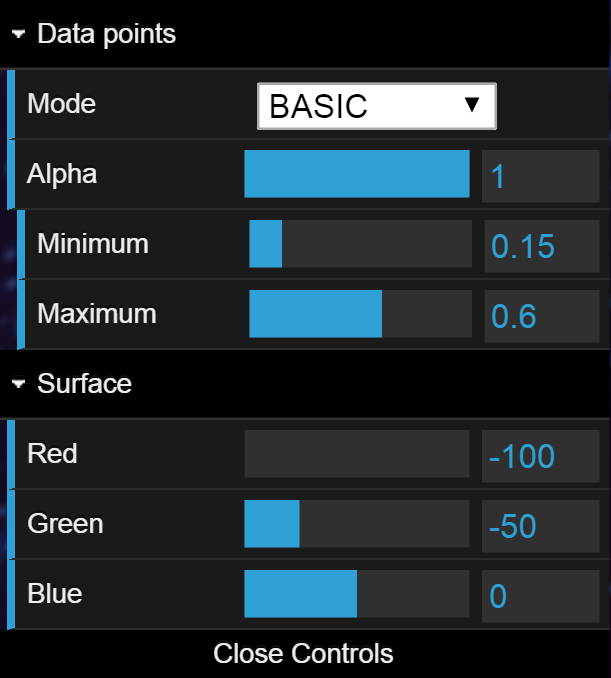
\includegraphics[width=\textwidth,height=\figureheight]{images/implementation/dat_gui/before}}
		\caption{Original dat.GUI interface.}
		\label{fig:dat_gui_before}
	\end{subfigure}
	\begin{subfigure}[b]{\figurewidth}
		\figureborder{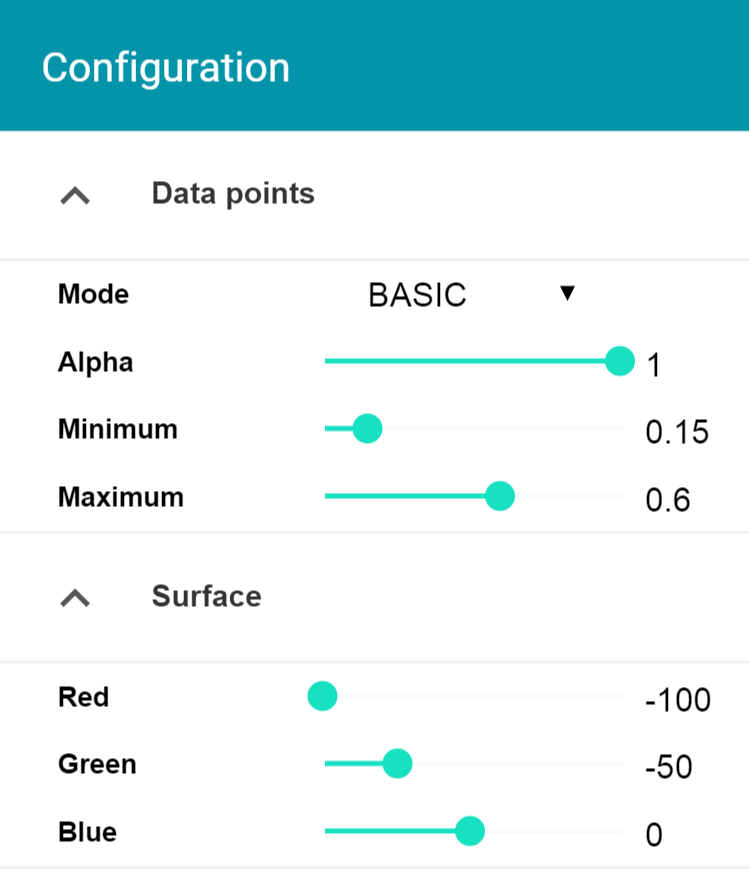
\includegraphics[width=\textwidth,height=\figureheight]{images/implementation/dat_gui/after}}
		\caption{dat.GUI interface after custom styling.}
		\label{fig:dat_gui_after}
	\end{subfigure}
	\caption[dat.GUI interface]{dat.GUI interface.}
	\label{fig:dat_gui}
\end{figure}


	The design for these configurations were continually refined during implementation. Initially, the dat.GUI sliders were to remain unchanged. However, these sliders proved to be inconsistent in regards to the colour scheme and filter design. Furthermore, the bold folder colours were eventually removed to reflect drawer layouts that conform to using light navigation colours, hover effects, and left floated icons.

}

Three inheritance-based visualisations were developed to demonstrate the potential of geovisualisations and how they can be applied to different datasets. Each visualisation utilises common navigation techniques, information displays for the data displays, filtering and configurable environment settings. Lastly, these features have been developed to provide the user with a range of tools for analysing the data presented to them.
